\documentclass[a4paper]{article}  

\usepackage{mathtools}
\usepackage{amsthm}
\usepackage{amssymb}
\usepackage{tikz}
\usepackage{algpseudocode}

\title{CS270 Homework 4}
\author{Valkyrie Savage \thanks{Shiry, Mitar, Orianna, Peggy, Jan Vondr\'{a}k of Stanford, S\'{e}bastien Lahaie of Columbia, stat.ethz.ch, Wikipedia}}

\begin{document}
\maketitle

\begin{enumerate}

\item Maximum weight bipartite matching
	\begin{enumerate}
		\item For example:\\
		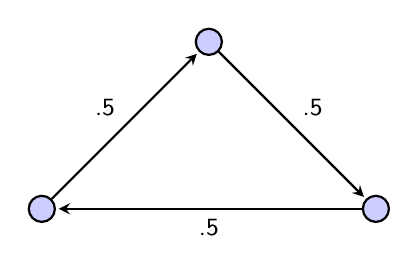
\begin{tikzpicture}[->,>=stealth,shorten >=1pt,auto,node distance=3cm,
 		thick,main node/.style={circle,fill=blue!20,draw,font=\sffamily\Large\bfseries}]

  		\node[main node] (B) {};
  		\node[main node] (A) [below left of=B] {};
  		\node[main node] (C) [below right of=B] {};

  		\path[every node/.style={font=\sffamily\small}]
    		(A) edge node {.5} (B)
        		(B) edge node {.5} (C)
        		(C) edge node {.5} (A);
		\end{tikzpicture}
		\item 
			\begin{align}
				\max \sum_e{w_e x_e}\\
				\forall v \in V : \sum_{e=(u,v)} {x_e} &\leq 1 \\
				 \forall S \subseteq V s.t. \left| {S} \right| odd :
					\sum_{C(S, \overline{S})}{x_e} & \geq 1 \\
				x_e &\geq 0
			\end{align}
		\item We get the dual of the linear program by creating one dual variable per constraint.  For the first constraint, we note that we are adding each edge twice, once when it appears for the endpoint $u$ and once when it appears for the endpoint $v$, so we have $y_u,y_v$.  In the second constraint, we have $\tilde{y_S}$, which appears once each time an edge falls across a cut (defined by the set $cutsacross(e)$).  Our dual objective function minimizes across all the vertices we see and all the oddcut sets.  The result is this :
			\begin{align}
				\min \sum_{v \in V}{y_v} - \sum_{S \in oddcuts}{\tilde{y_S}} \\
				\forall e = (u,v) \in E :: w_e \leq y_v + y_u - \sum_{S \in cutsacross(e)}{\tilde{y_S}}
			\end{align}
	\end{enumerate}
	A nice interpretation of this is XXXX????
\item Convex bodies
	\begin{enumerate}
		\item We have two bodies, $A$ and $B$.  We select a point $a \in A$ where $a$ is the closest point in $A$ to $B$ and a point $b \in B$ where $b$ is the closest point in $B$ to $A$.  We construct a hyperplane between $a$ and $b$.  If the hyperplane intersects $A$ at a point $a_1$, then we know that $a$ was not, in fact, the closest point in $A$ to $B$.  Similarly, if the hyperplane intersects $B$ at a point $b_1$, then we know that $b$ was not, in fact, the closest point in $B$ to $A$.
		\item Farkas B states that there is a solution for exactly one of
			\begin{enumerate}
				\item $Ax \leq b$
				\item $y^TA=0, y^Tb<0, y \geq 0$
			\end{enumerate}
			Both of these cannot be true, for the following reason:
			\begin{align}
				Ax &\leq b \\
				y^TAx &\leq y^Tb \\
				0 = y^TAx &\leq y^Tb <0 \\
				0 &< 0
			\end{align}
			One of them must be true, because if we assume that ii is not true, then i is true.  Either $y^TA < 0$ or $y^TA > 0$.  If $y^TA < 0$, we can construct some $b, y$ s.t. $y^TA \leq y^Tb$:
			\begin{align}
				y^TA &\leq y^Tb \\
				A &\leq b \\
			\end{align}
			So we can construct some $x$ s.t. $Ax \leq b$ (for example the identity). \\
			If $y^TA > 0$:
			\begin{align}
				y^TA &> y^Tb \\
				A &> b \\
			\end{align}
			It is not true that $\forall x : Ax \leq b$.
	\end{enumerate}

\item Facility Location
	\begin{enumerate}
		\item F and C, give C'
		\item find a facility location
		\item consider the distances 1 or 3
	\end{enumerate}
\item Relational database joins

\item Project description \\
	Working with Mitar to analyze/illustrate multi-way voting algorithms.
\end{enumerate}
\end{document}